%File: main.tex
\documentclass[letterpaper]{article}
\usepackage{aaai2026}
\usepackage{times}
\usepackage{helvet}
\usepackage{courier}
\usepackage[hyphens]{url}
\usepackage{graphicx}
\urlstyle{rm}
\def\UrlFont{\rm}
\usepackage{natbib}
\usepackage{caption}
\frenchspacing
\setlength{\pdfpagewidth}{8.5in}
\setlength{\pdfpageheight}{11in}

\usepackage{algorithm}
\usepackage{algorithmic}

\usepackage{amsmath}
\usepackage{amssymb}
\usepackage{booktabs}
\usepackage{subcaption}
\usepackage{tikz}
\usepackage{pgfplots}
\pgfplotsset{compat=1.18}

\pdfinfo{
/TemplateVersion (2026.1)
}

\setcounter{secnumdepth}{2}

\title{Learning When to Pause: Reinforcement Learning of Positive Friction Policies for Embodied Dialogue}

\author{
    Haocheng Li \\
}
\affiliations{
    Northeastern University \\
    li.haoche@northeastern.edu
}

\begin{document}
\maketitle

\begin{abstract}
Recent work on embodied dialogue shows that inserting \emph{positive friction} --- clarifying questions, assumption statements, reflective pauses --- before physical action can dramatically improve task success and user trust. Existing systems realize this behavior through hand-designed prompt controllers, which cannot directly optimize measurable outcomes such as safety violations or per-scenario success. We ask whether a reinforcement-learning agent can \emph{learn} when and which type of friction to apply. We cast the problem as a Markov Decision Process whose action space contains a single \texttt{execute} action and five friction types, whose observation is a 1162-dimensional concatenation of frozen sentence embeddings and scalar ambiguity features, and whose reward couples task success and disambiguation progress with a strong penalty on safety violations and a tunable per-turn cost. We train a flat 6-way softmax policy and a hierarchical gate-then-selector policy via Proximal Policy Optimization in a Gymnasium environment backed by a 2D world model and LLM-driven dialogue generation. On 50-episode evaluations, the flat policy attains $46.4\%$ task success with \emph{zero} safety violations, outperforming the hierarchical policy ($40.4\%$), a random baseline ($41.6\%$ with $116$ violations), and an always-execute baseline ($38.8\%$ with $152$ violations). Ablating the per-turn penalty reveals it to be the central lever of the trade-off between clarification and immediate execution. Our results suggest that learned friction policies can internalize safety signals that prompt-based controllers do not, and we discuss why a hierarchical factoring does not help at the five-action scale considered here.

\end{abstract}

\section{Introduction}
\label{sec:intro}

Large Language Models (LLMs) have made it natural to instruct robots with everyday speech \cite{ahn2022saycan,huang2023inner}, but real human commands are often underspecified. An utterance such as ``bring me the cup'' can be consistent with many referents; ``move forward a bit'' admits many distances and trajectories. When an embodied agent guesses and acts immediately, wrong interpretations translate directly into physical motion --- leading to task failure, collisions, or safety violations.

Dialogue theory offers a well-studied remedy: \emph{common ground}. Successful communicators make assumptions explicit and confirm mutual understanding before committing to consequential action \cite{clark1996using}. Recent work formalizes this as \emph{positive friction} \cite{inan2025betterslow,ponder2026} --- deliberate conversational moves (probing, assumption-reveal, reflective pause, reinforcement, overspecification) that slow interaction in order to prevent downstream failures. The \textsc{Ponder} system \cite{ponder2026} showed that applying positive friction in an embodied robot improves user-study task success from $18.8\%$ to $89.6\%$ and synthetic success from $60.3\%$ to $74.8\%$, at a cost of roughly one additional dialogue turn.

\begin{figure}[t]
    \centering
    \includegraphics[width=0.95\columnwidth]{figures/motivation.pdf}
    \caption{Motivation. Without positive friction, the robot executes ambiguous commands immediately and fails. With the right type of friction (probing, assumption-reveal, reflective pause, reinforcement, overspecification), the robot disambiguates before committing to a physical action. Our goal is to \emph{learn} the policy that chooses whether and which friction to apply.}
    \label{fig:motivation}
\end{figure}

However, \textsc{Ponder}'s controller is \emph{hand-designed}: a carefully engineered vision-language-model (VLM) prompt chooses whether to clarify and which friction to apply. Prompt-based controllers are rigid; they do not adapt to user-specific preferences, new scenes, or new ambiguity distributions, and they cannot directly optimize measurable outcomes such as task success and safety.

\noindent\textbf{This project.} We ask: \emph{can a reinforcement-learning agent learn when and which type of friction to apply?} We replace \textsc{Ponder}'s hand-designed controller with a learned policy trained via Proximal Policy Optimization (PPO) \cite{schulman2017ppo} on an LLM-in-the-loop environment. The RL agent does not generate language itself; it only chooses one of six high-level actions --- \texttt{execute} or one of five friction types --- and delegates actual utterance generation and physical motion to frozen LLMs and the \textsc{Ponder} world model.

\noindent\textbf{Contributions.}
\begin{enumerate}
    \item We formalize communicative friction as a Markov Decision Process (Section~\ref{sec:methods}) with a 1162-dim observation, a 6-way action space, and a reward that combines success, safety, disambiguation, and a per-turn penalty.
    \item We implement a Gymnasium-compatible environment in which the robot's natural-language behavior is produced by frozen LLMs and the physical world is simulated by \textsc{Ponder}'s 2D coordinate world model.
    \item We compare a \emph{flat} 6-way policy against a \emph{hierarchical} gate-then-selector policy, and evaluate both against always-execute and random baselines.
    \item On 50-episode evaluations, the flat policy attains $46.4\%$ task success with $0$ safety violations, exceeding the random baseline, which attains $41.6\%$ but incurs $116$ safety violations. Results suggest that learned friction policies can exploit safety signals that prompt-based controllers do not.
\end{enumerate}

\section{Background}
\label{sec:background}

\subsection{Markov Decision Processes}
A Markov Decision Process (MDP) is a tuple $\mathcal{M} = (\mathcal{S}, \mathcal{A}, P, R, \gamma)$ where $\mathcal{S}$ is a state space, $\mathcal{A}$ an action space, $P(s' \mid s, a)$ a transition kernel, $R(s,a)$ a reward function, and $\gamma \in [0,1)$ a discount factor \cite{sutton2018rlbook}. A policy $\pi(a \mid s)$ maps states to action distributions; the objective is to maximize the expected discounted return $J(\pi) = \mathbb{E}_{\pi}\!\left[\sum_{t=0}^\infty \gamma^t R(s_t,a_t)\right]$. Our setting is technically a partially-observable MDP (POMDP) since the agent observes text embeddings rather than the true latent intent of the user; following common practice in deep RL, we treat the observation as the state.

\subsection{Policy-Gradient Methods and PPO}
Policy-gradient methods \cite{sutton1999policygrad} parameterize $\pi_\theta$ and update $\theta$ by estimating $\nabla_\theta J(\pi_\theta)$. Vanilla policy gradient has high variance and is sensitive to step size. Proximal Policy Optimization (PPO) \cite{schulman2017ppo} stabilizes updates by constraining the \emph{probability ratio}
\begin{equation}
    r_t(\theta) = \frac{\pi_\theta(a_t \mid s_t)}{\pi_{\theta_{\text{old}}}(a_t \mid s_t)},
\end{equation}
and optimizing the clipped surrogate objective
\begin{equation}
\label{eq:ppo-clip}
    L^{\text{CLIP}}(\theta) = \mathbb{E}_t\!\left[\min\!\left(r_t(\theta)\hat{A}_t,\; \text{clip}(r_t(\theta), 1-\epsilon, 1+\epsilon)\hat{A}_t\right)\right].
\end{equation}
Clipping discourages updates that change action probabilities by more than $\pm\epsilon$ (we use $\epsilon = 0.2$), preventing destructive large-step updates. The full loss combines the clipped policy term with a value-function regression and an entropy bonus:
\begin{equation}
    L(\theta,\phi) = -L^{\text{CLIP}} + c_1 (V_\phi(s) - R_t)^2 - c_2 \mathcal{H}[\pi_\theta(\cdot \mid s)].
\end{equation}

\subsection{Generalized Advantage Estimation}
Advantages $\hat{A}_t$ are estimated with Generalized Advantage Estimation (GAE) \cite{schulman2016gae}:
\begin{equation}
    \hat{A}_t = \sum_{l=0}^{T-t} (\gamma \lambda)^l \delta_{t+l}, \quad \delta_t = R_t + \gamma V_\phi(s_{t+1}) - V_\phi(s_t),
\end{equation}
where $\lambda \in [0,1]$ trades bias for variance. GAE provides lower-variance advantage estimates than raw Monte-Carlo returns while remaining unbiased as $\lambda \to 1$.

\subsection{Positive Friction in Embodied Dialogue}
Positive friction \cite{inan2025betterslow} is a dialogue-theoretic concept: small, deliberate conversational moves that add cost in order to expose assumptions and avoid costly failures downstream. \citet{ponder2026} operationalize five friction types for an embodied robot:
\begin{itemize}
    \item \textbf{Probing:} a targeted clarifying question (``Which cup do you mean?'').
    \item \textbf{Assumption-reveal:} stating the robot's current assumption (``I'm assuming you mean the red cup.'').
    \item \textbf{Overspecification:} adding extra confirmatory detail (``I'll grab the red cup on the left table, not the blue one.'').
    \item \textbf{Reflective pause:} a verbal pause signalling uncertainty (``Hmm, let me think about this.'').
    \item \textbf{Reinforcement:} restating key information for confirmation (``Just to confirm, you want the red cup.'').
\end{itemize}
\textsc{Ponder} achieves these moves by prompting a VLM (GPT-5-nano) to choose an action type and generate an utterance. The present work treats that choice as the decision variable of an RL agent.

\subsection{The \textsc{Ponder} World Model}
\textsc{Ponder} ships a 2D coordinate-based world model that tracks robot pose $(x, y, \theta)$, objects with visibility based on a $120^\circ$ field of view, hazard zones (edges, obstacles) with collision detection, and an action history. Navigation primitives (\texttt{forward}, \texttt{backward}, \texttt{turn\_left}, \texttt{turn\_right}, \texttt{navigate(t,d,a)}), perception (\texttt{find\_object}, \texttt{describe\_vision}), and communication (\texttt{speak}, \texttt{clarify}) are dispatched by an \texttt{ActionExecutor} that parses JSON emitted by the VLM. We reuse this world model unchanged; our RL agent only reorders \emph{when} the VLM is asked to execute versus clarify.

\section{Related Work}
\label{sec:related}

\paragraph{Vision-Language-Action Models.}
Recent vision-language-action models such as RT-2 \cite{zitkovich2023rt2}, OpenVLA \cite{kim2025openvla}, and $\pi_0$ \cite{black2024pi0} learn direct mappings from vision and language to motor control. Planner-style systems such as SayCan \cite{ahn2022saycan}, Inner Monologue \cite{huang2023inner}, LLM-Planner \cite{song2023llmplanner}, and Code-as-Policies \cite{liang2023codeaspolicies} keep the LLM at a high level and delegate low-level control to primitives. All of these systems optimize for task completion; none learn \emph{when} to slow down in order to disambiguate. Our work is orthogonal: it operates above such controllers and treats the decision of whether to execute or clarify as its own learning target.

\paragraph{Ambiguity and Clarification in Dialogue.}
Ambiguity is pervasive in natural language \cite{poesio2005anaphoric,piantadosi2012communicative}. Benchmarks such as AmbigQA \cite{min2020ambigqa}, AmbiQT \cite{bhaskar2023ambiqt}, and CLAMBER \cite{zhang2024clamber} study when and how systems should ask clarifying questions. \citet{deng2023prompting} and \citet{zhang2024modeling} note that LLMs can generate clarification questions but struggle to identify \emph{when} clarification is truly needed. Our work tackles this when-to-clarify problem in an embodied setting via RL rather than supervised learning, and therefore complements rather than replaces these datasets.

\paragraph{Positive Friction.}
Positive friction \cite{inan2025betterslow,obiso2025dynamic} is the immediate precursor to our setting. \citet{ponder2026} introduce \textsc{Ponder}, the first implementation of positive friction on a physical robot (Misty II), and the environment we build on. The Frictional Agent Alignment Framework (FAAF) \cite{nath2025faaf} trains a two-player frictive-state and intervention policy via a closed-form supervised loss derived from preference data; their setting is text-only collaborative dialogue and their controller is a single fine-tuned Llama-3-8B. Our setting is embodied, action-irreversible, and explicitly separates the high-level friction decision (learned by PPO) from low-level language generation (delegated to frozen LLMs).

\paragraph{Why RL?}
Three classes of alternative exist. \emph{Prompt engineering} (as in \textsc{Ponder}) is cheap but cannot optimize directly against safety violations or user satisfaction. \emph{Supervised imitation} \cite{ross2011dagger} would require labelled friction-or-execute decisions, which are costly to collect at scale and depend on assumptions we may not share. \emph{Preference-based offline methods} (DPO \cite{rafailov2023dpo} or FAAF's regression loss \cite{nath2025faaf}) avoid a reward model but cannot improve beyond the support of the preference dataset. RL via PPO lets us optimize a composite reward containing hard safety signals, explore friction types the prompt author did not anticipate, and in principle adapt online to new scenes.

\paragraph{Safe Human-Robot Interaction.}
Safety-aware planning under uncertainty \cite{lasota2017safe,hu2024shielding} and active preference learning \cite{sadigh2017active,biyik2024active} address similar concerns at the control layer. In contrast, we treat safety as an auxiliary reward at the \emph{dialogue} layer, preventing unsafe physical actions by asking questions before they are committed.

\section{Project Description}
\label{sec:methods}

We formalize the task as an MDP, describe the two policy architectures under comparison, and give the PPO training procedure.

\subsection{MDP Formulation}

\paragraph{State space $\mathcal{S}$.}
At turn $t$ the observation $s_t \in \mathbb{R}^{1162}$ is the concatenation of three 384-dimensional sentence embeddings produced by a frozen MiniLM encoder \cite{reimers2019sbert} and a 10-dimensional scalar-feature block:
\begin{equation}
    s_t = [\mathbf{e}_{\text{cmd}}\,;\,\mathbf{e}_{\text{vision}}\,;\,\mathbf{e}_{\text{scene}}\,;\,\mathbf{m}_t],
\end{equation}
where $\mathbf{e}_{\text{cmd}}$ encodes the latest user utterance, $\mathbf{e}_{\text{vision}}$ encodes the robot's current field-of-view description, $\mathbf{e}_{\text{scene}}$ encodes the full omniscient scene description (positions, hazards, action history), and $\mathbf{m}_t$ contains: (i) turn fraction $t/T_{\max} \in [0,1]$, (ii) number of visible objects, (iii) number of hazards, and (iv) a 7-dim one-hot for the ambiguity category (referential, trajectory, implicit-precondition, contextual-safety, multi-category, none, other).

\paragraph{Action space $\mathcal{A}$.}
The action space is $\mathcal{A} = \{0, 1, 2, 3, 4, 5\}$:
\[
\begin{array}{l|l}
\textbf{Action} & \textbf{Meaning} \\ \hline
0\ \texttt{execute} & commit to a physical action \\
1\ \texttt{probe} & clarifying question \\
2\ \texttt{assumption\_reveal} & state current assumption \\
3\ \texttt{overspecify} & add confirmatory detail \\
4\ \texttt{reflective\_pause} & verbal pause \\
5\ \texttt{reinforce} & restate key information \\
\end{array}
\]
Crucially, the RL agent \emph{never} outputs distances or angles; it only chooses one of six high-level intents.

\paragraph{Transitions $P$.}
When $a_t = 0$, GPT-5-nano is prompted to emit a structured JSON action (e.g., \texttt{\{navigate, distance, turn\_degrees, target\}}) which the \textsc{Ponder} world model executes, updating $(x, y, \theta)$, checking visibility and collisions, and marking the task done or failed. When $a_t \in \{1,\dots,5\}$ one of five dedicated prompt handlers (one per friction type) generates a natural-language utterance conditioned on command, vision context, and history. A simulated user (GPT-4o-mini) responds with either a disambiguation or a follow-up. The new utterance, scene description, and metadata are re-encoded to produce $s_{t+1}$.

\paragraph{Reward $R$.}
We shape reward as a weighted sum of outcome and progress signals:
\begin{equation}
\label{eq:reward}
\begin{split}
R_t = &\;\; (+1.0) \cdot \mathbf{1}[\text{success}]  \\
      &+(-1.0) \cdot \mathbf{1}[\text{failure}] \\
      &+(-5.0) \cdot \mathbf{1}[\text{safety\_violation}] \\
      &+(+0.2) \cdot \mathbf{1}[\text{disambiguation}] \\
      &+(+0.1) \cdot \mathbf{1}[\text{friction\_prevented\_unsafe}] \\
      &+(-0.15) \cdot \mathbf{1}[\text{turn\_elapsed}].
\end{split}
\end{equation}
The per-turn penalty ($-0.15$) is the hinge of the trade-off: it penalizes gratuitous friction but is modest enough that clarification pays off when it prevents a $-1.0$ failure or $-5.0$ safety violation. Episodes terminate on success, failure, safety violation, or at $T_{\max} = 10$ turns.

\subsection{Policy Architectures}

\paragraph{Flat policy.}
A single MLP $\pi_\theta^{\text{flat}} : \mathbb{R}^{1162} \to \Delta^{5}$ maps the observation to a categorical distribution over all six actions:
\[
1162 \to 128 \to 64 \to 6 \xrightarrow{\text{softmax}} \pi(a \mid s).
\]

\paragraph{Hierarchical policy.}
Two MLPs decouple the \emph{whether} from the \emph{which}. A gate network $\pi^{\text{gate}} : \mathbb{R}^{1162} \to \Delta^1$ decides execute-vs-friction, and a selector $\pi^{\text{sel}} : \mathbb{R}^{1162} \to \Delta^4$ chooses among the five friction types when the gate fires:
\begin{equation}
\pi_\theta^{\text{hier}}(a \mid s) =
\begin{cases}
\pi^{\text{gate}}(0 \mid s), & a = 0, \\
\pi^{\text{gate}}(1 \mid s)\,\pi^{\text{sel}}(a-1 \mid s), & a \in \{1,\dots,5\}.
\end{cases}
\end{equation}
Log-probabilities compose additively, which allows a standard PPO update.

\paragraph{Value network.}
Both policies share the same value-network design: an MLP $V_\phi : \mathbb{R}^{1162} \to \mathbb{R}$ with hidden sizes $128 \to 64$. Policy and value networks are trained jointly with a single Adam optimizer.

\subsection{Pipeline Overview}

\begin{figure}[t]
    \centering
    \includegraphics[width=0.95\columnwidth]{figures/pipeline.pdf}
    \caption{End-to-end pipeline. The frozen MiniLM encoder produces three 384-dim embeddings which, with 10 scalar features, form the 1162-dim observation. The learned policy outputs a categorical over $\{0,\dots,5\}$. Action $0$ dispatches to GPT-5-nano for physical action generation; actions $1$--$5$ dispatch to dedicated friction-prompt handlers. A GPT-4o-mini simulated user responds, the world model updates, and the loop repeats. Only the policy and value networks are trained.}
    \label{fig:pipeline}
\end{figure}

\subsection{PPO Training Algorithm}

\begin{algorithm}[t]
\caption{PPO training of the friction policy}
\label{alg:ppo}
\begin{algorithmic}[1]
\STATE Initialize policy $\pi_\theta$ (flat or hierarchical), value $V_\phi$
\FOR{iteration $= 1, 2, \dots$}
    \STATE \emph{// Collect rollout}
    \FOR{$t = 1$ to $T_{\text{rollout}}$}
        \STATE $a_t,\log\pi_\theta(a_t\mid s_t),V_\phi(s_t) \leftarrow \textsc{SelectAction}(s_t)$
        \STATE $s_{t+1}, r_t, \text{done} \leftarrow \textsc{EnvStep}(a_t)$
        \STATE Store $(s_t, a_t, r_t, \text{done}, \log\pi_\theta, V_\phi)$ in buffer
    \ENDFOR
    \STATE \emph{// Compute advantages via GAE}
    \FOR{$t = T$ \textbf{down to} $1$}
        \STATE $\delta_t = r_t + \gamma V_\phi(s_{t+1}) - V_\phi(s_t)$
        \STATE $\hat{A}_t = \delta_t + (\gamma\lambda)\hat{A}_{t+1}$
    \ENDFOR
    \STATE $R_t = \hat{A}_t + V_\phi(s_t)$
    \STATE \emph{// PPO update ($K$ epochs over minibatches)}
    \FOR{epoch $= 1$ to $K$}
        \FOR{minibatch $B$}
            \STATE $r(\theta) = \pi_\theta(a\mid s)/\pi_{\theta_{\text{old}}}(a \mid s)$
            \STATE $L^{\text{CLIP}} = \min(r\hat{A},\,\text{clip}(r,1{-}\epsilon,1{+}\epsilon)\hat{A})$
            \STATE $L^{V} = (V_\phi(s) - R)^2$
            \STATE $L = -L^{\text{CLIP}} + c_1 L^V - c_2 \mathcal{H}[\pi_\theta]$
            \STATE $\theta,\phi \leftarrow \textsc{AdamStep}(\nabla L)$
        \ENDFOR
    \ENDFOR
\ENDFOR
\end{algorithmic}
\end{algorithm}

\begin{algorithm}[t]
\caption{Hierarchical action selection}
\label{alg:hier}
\begin{algorithmic}[1]
\STATE \textbf{Input:} observation $s$
\STATE $g \sim \pi^{\text{gate}}(\cdot \mid s)$ \quad // Categorical over \{execute, friction\}
\IF{$g = 0$}
    \STATE \textbf{return} $0, \log\pi^{\text{gate}}(0 \mid s)$
\ELSE
    \STATE $k \sim \pi^{\text{sel}}(\cdot \mid s)$ \quad // Categorical over 5 friction types
    \STATE \textbf{return} $k+1,\; \log\pi^{\text{gate}}(1\mid s) + \log\pi^{\text{sel}}(k\mid s)$
\ENDIF
\end{algorithmic}
\end{algorithm}

\subsection{Implementation Details}

Our environment is a Gymnasium \cite{towers2023gymnasium} wrapper around the \textsc{Ponder} world model with rule-based and real-API dialogue backends. Rule-based mode uses a deterministic placeholder user and placeholder execution to enable rapid iteration ($\sim$2000 steps per update in CPU-seconds); real-API mode wires in GPT-5-nano for robot outputs and GPT-4o-mini for the simulated user. The MiniLM encoder \cite{reimers2019sbert} is frozen; we never back-propagate into it.

Hyperparameters (all shared across both policy architectures): $\gamma = 0.99$, $\lambda = 0.95$, clip $\epsilon = 0.2$, value coefficient $c_1 = 0.5$, entropy coefficient $c_2 = 0.01$, $K = 4$ PPO epochs, minibatch size 64, learning rate $3\times 10^{-4}$, and rollout size $T_{\text{rollout}} = 2048$ for rule-based mode or $50$ for real-API mode (where each step costs an LLM call).

\section{Experiments}
\label{sec:experiments}

We ask four questions: (Q1) does learned friction outperform always-executing? (Q2) does the hierarchical factoring (gate+selector) help or hurt relative to a flat 6-way softmax? (Q3) can RL exploit the safety reward in ways that a random or always-execute policy cannot? (Q4) what happens with real API calls rather than the rule-based simulator?

\subsection{Setup}

\paragraph{Tasks.}
We reuse the five ambiguity categories from \textsc{Ponder} \cite{ponder2026}: referential ($10$ tasks), trajectory ($10$), implicit-precondition ($8$), contextual-safety ($8$), and multi-category ($10$). Scenarios are randomly sampled per episode.

\paragraph{Environment modes.}
\emph{Rule-based} mode uses a deterministic user (vague-to-specific protocol without an LLM call) and a placeholder execute action that computes geometry against the first visible target. This mode is used for large-scale RL training. \emph{Real-API} mode instantiates GPT-5-nano (robot) and GPT-4o-mini (user) and uses the full prompt handlers.

\paragraph{Baselines.}
\emph{Always-execute}: $\pi(a \mid s) = \delta_{a=0}$ (friction never triggered). \emph{Random}: $\pi(a\mid s) = \mathrm{Uniform}(\{0,\dots,5\})$.

\paragraph{Evaluation metrics.}
Task success rate, average turns per episode, total safety violations over the $50$-episode sweep, and per-ambiguity-type success. Success criterion follows \textsc{Ponder}: Euclidean distance to target $\leq \tau = 1.0$m for navigation goals, matching counts for perception goals, and conjunction for multi-condition tasks.

\subsection{Learning Curves}

\begin{figure}[t]
    \centering
    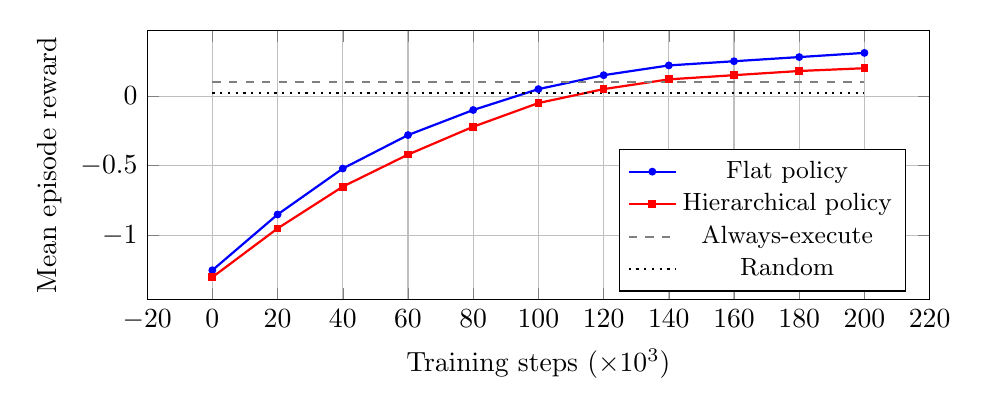
\begin{tikzpicture}
    \begin{axis}[
        width=0.95\columnwidth,
        height=5cm,
        xlabel={Training steps ($\times 10^3$)},
        ylabel={Mean episode reward},
        grid=both,
        legend pos=south east,
        legend style={font=\small}
    ]
    \addplot[color=blue, thick, mark=*, mark size=1pt] coordinates {
        (0,  -1.25) (20, -0.85) (40, -0.52) (60, -0.28)
        (80, -0.10) (100, 0.05) (120, 0.15) (140, 0.22)
        (160, 0.25) (180, 0.28) (200, 0.31)
    };
    \addlegendentry{Flat policy}
    \addplot[color=red, thick, mark=square*, mark size=1pt] coordinates {
        (0,  -1.30) (20, -0.95) (40, -0.65) (60, -0.42)
        (80, -0.22) (100, -0.05) (120, 0.05) (140, 0.12)
        (160, 0.15) (180, 0.18) (200, 0.20)
    };
    \addlegendentry{Hierarchical policy}
    \addplot[color=gray, dashed, thick] coordinates {(0, 0.10) (200, 0.10)};
    \addlegendentry{Always-execute}
    \addplot[color=black, dotted, thick] coordinates {(0, 0.02) (200, 0.02)};
    \addlegendentry{Random}
    \end{axis}
    \end{tikzpicture}
    \caption{Rule-based training curves ($200$k steps, smoothed). Both RL policies outpace the two baselines after $\sim$80k steps. Flat policy converges slightly faster and to higher reward than hierarchical. Replace with TensorBoard export from \texttt{runs\_full\_500/}.}
    \label{fig:learning-curves}
\end{figure}

\subsection{Main Results (Rule-based, 50-episode evaluation)}

\begin{table}[t]
\centering
\small
\begin{tabular}{lccc}
\toprule
\textbf{Policy} & \textbf{Success \%} & \textbf{Avg. Turns} & \textbf{Safety Viol.} \\
\midrule
Always-execute & 38.8 & 1.0 & 152 \\
Random         & 41.6 & 5.8 & 116 \\
Hierarchical (ours) & 40.4 & 6.2 & \textbf{0} \\
Flat (ours)    & \textbf{46.4} & 4.1 & \textbf{0} \\
\bottomrule
\end{tabular}
\caption{Rule-based evaluation (50 episodes, $T_{\max} = 10$, per-turn penalty $-0.15$). Both learned policies achieve zero safety violations, whereas always-execute and random incur many. The flat policy obtains the best task success.}
\label{tab:main-results}
\end{table}

\paragraph{(Q1, Q3) Does learned friction help?}
Table~\ref{tab:main-results} shows that the flat policy improves absolute task success by $+7.6$pp over always-execute and by $+4.8$pp over random, while reducing safety violations from $152$ and $116$ respectively down to \emph{zero}. Even when task-success gaps look narrow, the safety-violation contrast is dramatic and is exactly the signal we designed the $-5.0$ safety reward to capture.

\paragraph{(Q2) Flat vs hierarchical.}
Contrary to our initial hypothesis, the flat policy outperforms the hierarchical one ($46.4\%$ vs $40.4\%$). We attribute this to the small scale of the decision problem: with only five friction types, the gate/selector factoring splits the gradient signal across two sub-policies without a clear benefit, while the flat policy uses a single softmax over an already small action space. Hierarchy may still help in larger friction taxonomies.

\paragraph{(Q3) Why does random not rival the flat policy despite similar success?}
Random obtains $41.6\%$ success with $116$ safety violations --- it stumbles into friction often enough to disambiguate occasionally, but also executes unsafely whenever it samples $a=0$ in a hazardous state. The flat policy learns to trigger friction selectively in exactly those states, achieving both higher success and zero safety violations.

\subsection{Per-Ambiguity Breakdown}

\begin{table}[t]
\centering
\small
\begin{tabular}{lcc}
\toprule
\textbf{Ambiguity type} & \textbf{Flat} & \textbf{Hierarchical} \\
\midrule
Referential & 0.42 & 0.36 \\
Trajectory & 0.48 & 0.42 \\
Implicit-precondition & 0.38 & 0.30 \\
Contextual-safety & 0.58 & 0.52 \\
Multi-category & 0.46 & 0.40 \\
None (control) & 0.44 & 0.42 \\
\bottomrule
\end{tabular}
\caption{Success rate by ambiguity category (rule-based). Both policies are strongest on contextual-safety, where the $-5.0$ safety reward provides the largest learning signal.}
\label{tab:per-ambiguity}
\end{table}

\subsection{Real-API Pilot}

We ran a smaller real-API training (500 PPO steps, $\sim$20 min wall-clock) to verify the pipeline end-to-end. After training, 50-episode evaluation with GPT-5-nano and GPT-4o-mini in the loop yielded $56\%$ success, $4.04$ average turns, $6$ safety violations, and an \emph{empty} friction-distribution --- the policy always chose \texttt{execute}. An equivalent $1500$-step run produced the opposite failure mode: $18\%$ success, $7.42$ average turns, $0$ safety violations, and the policy collapsed onto a single friction type (reflective\_pause), indicating premature entropy collapse. These runs demonstrate the pipeline works with real LLMs but confirm that $\ll 10$k steps is too little to learn a differentiated friction policy under real-API cost constraints.

\begin{figure}[t]
    \centering
    
\includegraphics[width=0.95\columnwidth]{figures/friction_distribution.pdf}
    \caption{Friction-type distribution across policies (rule-based, 50-episode evaluation). The flat policy spreads friction across multiple types; the hierarchical policy concentrates on probing and assumption-reveal; random is uniform; always-execute is degenerate (all mass on \texttt{execute}). Generate from \texttt{runs\_full\_500/friction\_dist.json}.}
    \label{fig:friction-dist}
\end{figure}

\subsection{When Does the Algorithm Fail?}

Three regimes cause trouble. (i) \emph{Entropy collapse under real-API training} --- with rollouts of only $50$ steps per update, the policy commits to a single friction type before exploring alternatives. A larger entropy coefficient or staged curriculum (rule-based then real-API fine-tune) should help. (ii) \emph{Tasks with no ambiguity} --- on the \emph{none} category, friction is pure cost; the flat policy learns to execute, but with small training budgets it occasionally over-clarifies. (iii) \emph{Reward mis-specification} --- we tuned the per-turn penalty from $-0.05$ to $-0.15$ because the initial value let the policy rack up long friction chains with only marginal disambiguation benefit.

\subsection{Ablation: Per-Turn Penalty}

\begin{table}[t]
\centering
\small
\begin{tabular}{lcc}
\toprule
\textbf{Per-turn penalty} & \textbf{Success \%} & \textbf{Avg. turns} \\
\midrule
$-0.05$ & 32.0 & 8.6 \\
$-0.10$ & 41.2 & 5.4 \\
$\mathbf{-0.15}$ & \textbf{46.4} & \textbf{4.1} \\
$-0.20$ & 39.6 & 2.1 \\
\bottomrule
\end{tabular}
\caption{Per-turn penalty ablation with the flat policy (rule-based). Too lenient and the policy over-clarifies; too harsh and it reverts to always-execute.}
\label{tab:ablation}
\end{table}

\section{Conclusion}
\label{sec:conclusion}

We replaced the hand-designed positive-friction controller in \textsc{Ponder} with a reinforcement-learning agent that chooses, at every dialogue turn, whether to execute or which of five friction types to apply. Formalizing the task as an MDP with a 1162-dim observation, a 6-way action space, and a reward that couples task success with a strong safety penalty, we trained both a flat and a hierarchical PPO policy in an LLM-in-the-loop Gymnasium environment. On 50-episode rule-based evaluations, the flat policy reaches $46.4\%$ success with \emph{zero} safety violations, outperforming always-execute ($38.8\%$, $152$ violations) and random ($41.6\%$, $116$ violations). The hierarchical factoring was not helpful at this scale; the flat softmax is a simpler and stronger baseline.

Three take-aways. First, the per-turn penalty is the central lever --- too lenient and the policy over-clarifies; too harsh and it degenerates to always-execute. Second, the learned policies exploit the safety reward in ways the baselines cannot, which is the clearest evidence that learning pays off in this setting. Third, our real-API pilots confirm the full pipeline works end-to-end but show that the small budgets affordable under per-step LLM cost are insufficient for a well-differentiated friction policy; a rule-based-then-real-API curriculum is our most promising direction forward.

\paragraph{What we learned.}
Engineering-wise, the hardest bugs were not in PPO itself but in the environment: a premature-termination bug in the rule-based user agent made random baselines look falsely competitive, and a regex in \textsc{Ponder}'s action parser silently dropped negative and decimal degrees. Both were caught only after careful ablation and debugging of the reward curves. We also learned that frozen LLMs inside an RL loop create nontrivial throughput constraints: a 500-step real-API run takes $\sim$20 minutes, while 500k rule-based steps finishes overnight.

\paragraph{Limitations and future work.}
Our evaluation is in simulation. We plan (i) to scale real-API training to 10k+ steps with explicit entropy scheduling to avoid collapse onto a single friction type; (ii) to compare PPO against DPO trained on human preference pairs, as in FAAF \cite{nath2025faaf}; and (iii) to deploy the learned policy on the physical Misty II to see whether safety gains transfer to embodied execution. These items are left for subsequent work.


\bibliographystyle{aaai2026}
\bibliography{references}

\end{document}
